After extracting the user's e-mails, we should be able to analyse the body of the e-mails. To do this we will need a syntactic parser in order to separate the different texts in tokens (in other words, to segment text into words, punctuation marks, etc.) and obtain different characteristics from them (such as their part of speech) for the purpose of being able to calculate the metrics explained in Section \ref{ssect:stymet}. To attain that objective, we are going to use the library spaCy.

\subsection{spaCy versus others syntactic parsers}

We have chosen spaCy as our syntactic parser against others for several reasons that we will explain below.

\begin{figure}[h]
	\centering%
	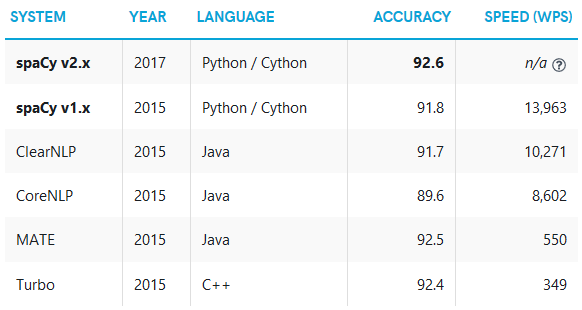
\includegraphics[width = 0.75\textwidth]{Imagenes/Bitmap/Spacy/spacyeval.png}%
	\caption{Benchmarks of different syntactic parsers}%
	Image extracted from \url{https://spacy.io/usage/facts-figures#benchmarks}
	\label{fig:spacyeval}
\end{figure}

An evaluation published by \textit{Yahoo! Labs} and Emory University, as a part of a survey of current parsing technologies \citep{choi2015depends}, observed that ``spaCy is the fastest greedy parser'' and its accuracy is within 1\% of the best available (as we can see in Figure \ref{fig:spacyeval}). The few systems that are more accurate are 20 times slower or more.

\cite{choi2015depends} results and subsequent discussions helped spaCy develop a novel psychologically-motivated technique to improve spaCy's accuracy, which they published in joint work with Macquarie University \citep{honnibal2015improved}.

Besides, not only in general but in each particular task (tokenisation, tagging and parsing), spaCy is the fastest if we compare it with other natural language processing libraries. This is shown in Figure \ref{fig:spacyspeed}, where we can observe both absolute timings (in ms) and relative performance (normalized to spaCy). Lower is better.

\begin{figure}[h]
	\centering%
	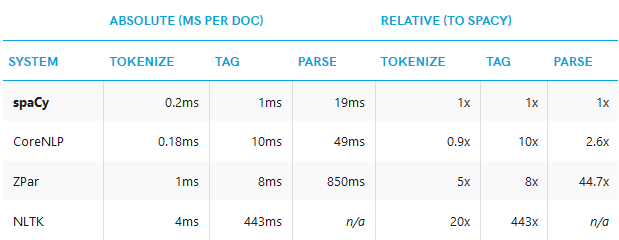
\includegraphics[width = 0.85\textwidth]{Imagenes/Bitmap/Spacy/spacyspeed.png}%
	\caption{Per-document processing time of various NLP libraries}%
	Image extracted from \url{https://spacy.io/usage/facts-figures#benchmarks}
	\label{fig:spacyspeed}
\end{figure}

Finally, spaCy has three pretrained model pipelines for Spanish with a very high accuracy (see Figure \ref{fig:spacymodel}). These will help us to tokenise, tag and parse our messages in order to calculate the different style markers defined.

\begin{figure}[h]
	\centering%
	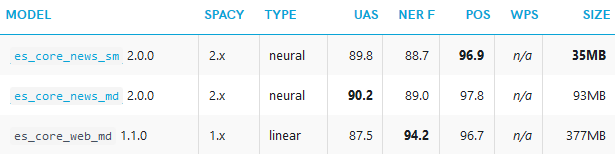
\includegraphics[width = 0.85\textwidth]{Imagenes/Bitmap/Spacy/spacymodel.png}%
	\caption{Benchmark accuracies for the Spanish pretrained model pipelines}%
	Image extracted from \url{https://spacy.io/usage/facts-figures#benchmarks}
	\label{fig:spacymodel}
\end{figure}